\documentclass{article}

\usepackage[spanish]{babel}
\usepackage[numbers,sort&compress]{natbib}
\usepackage{graphicx}
\usepackage{url}
\usepackage{amsmath}
\usepackage{hyperref}
\usepackage[top=30mm, bottom=40mm, left=15mm, right=15mm]{geometry}
\usepackage{listings}
\usepackage{subfig}
\usepackage{color}
\usepackage{multirow}
\usepackage[latin1]{inputenc}

\setlength{\parskip}{2mm}
\setlength{\parindent}{0pt}
\definecolor{dkgreen}{rgb}{0,0.6,0}
\definecolor{gray}{rgb}{0.3,0.3,0.3}
\definecolor{orange}{rgb}{0.8,0.4,0}
\definecolor{mostaza}{rgb}{0.9,0.8,0.1}

\lstset{ %
  language=R,                     % the language of the code
  basicstyle=\footnotesize,       % the size of the fonts that are used for the code
  numbers=left,                   % where to put the line-numbers
  numberstyle=\tiny\color{gray},  % the style that is used for the line-numbers
  stepnumber=1,                   % the step between two line-numbers. If it's 1, each line
                                  % will be numbered
  numbersep=5pt,                  % how far the line-numbers are from the code
  backgroundcolor=\color{white},  % choose the background color. You must add \usepackage{color}
  showspaces=false,               % show spaces adding particular underscores
  showstringspaces=false,         % underline spaces within strings
  showtabs=false,                 % show tabs within strings adding particular underscores
  frame=single,                   % adds a frame around the code
  rulecolor=\color{black},        % if not set, the frame-color may be changed on line-breaks within not-black text (e.g. commens (green here))
  tabsize=2,                      % sets default tabsize to 2 spaces
  captionpos=b,                   % sets the caption-position to bottom
  breaklines=true,                % sets automatic line breaking
  breakatwhitespace=false,        % sets if automatic breaks should only happen at whitespace
  title=\lstname,                 % show the filename of files included with \lstinputlisting;
                                  % also try caption instead of title
  keywordstyle=\color{orange},      % keyword style
  commentstyle=\color{dkgreen},   % comment style
  stringstyle=\color{mostaza},      % string literal style
  escapeinside={\%*}{*)},         % if you want to add a comment within your code
  morekeywords={*,...}            % if you want to add more keywords to the set
} 

\author{Marco Antonio Guajardo Vigil  2095}
\title{\textbf{Pr\'actica 9: Interacciones entre part\'iculas} \\ Simulaci\'on de sistemas}
\date{02 de abril, 2019}

\begin{document}

\maketitle

\section{Introducci\'on}
Se supone un modelo simplificado para los fen\'onemos de atracci\'on y repulsi\'on de f\'isica(o qu\'imica). Contamos con $n$ part\'iculas que habitan un cuadro unitario bidimensional y que cada part\'icula tiene una carga el\'ectrica, distribuida independientemente y normalmente al azar entre $[-1,1]$ \ref{fig:modelo}.

Cargas de un mismo signo producen una repulsi\'on mientras que cargas opuestas resultan en una atracci\'on, la magnitud de la fuerza est\'a proporcional a la diferencia de magnitud de las cargas (mayores diferencias resultan mayores fuerzas), y adem\'as la fuerza es inversamente proporcional a la distancia euclideana entre las part\'iculas \cite{SatuP9}.

\section{Objetivo}

Se agrega a cada part\'icula una \textbf{masa} y esta causa fuerzas gravitacionales (atracciones) adem\'as de las fuerzas causadas por las cargas. Se estudia la distribuci\'on de velocidades de las part\'iculas y se verifica gr\'aficamente que est\'e presente una relaci\'on entre los tres factores: la \textbf{velocidad}, la \textbf{magnitud de la carga} y \textbf{la masa de las part\'iculas}. La velocidad tambi\'en es afectada por las posiciones.

\begin{figure}[h!]
\centering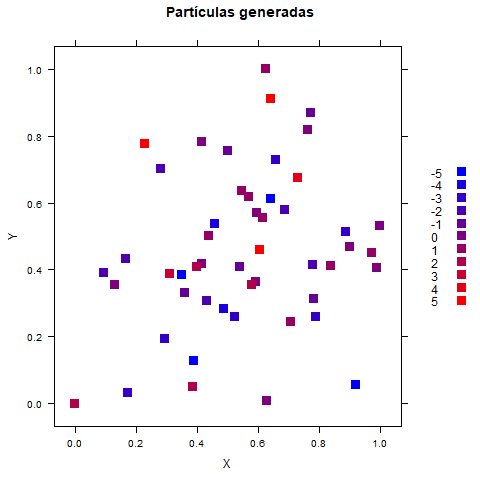
\includegraphics[width=60mm]{p9i.png}
\caption{Modelo bidimensional de part\'iculas con cargas el\'ectricas distribuidas al azar.}
\label{fig:modelo}
\end{figure}

\newpage

\subsection{Implementaci\'on de R}
Para la elaboraci\'on de este experimento, se hace uso de un software libre para computaci\'on estad\'istica y gr\'aficos llamado \citet{R}, el cual nos permite realizar los c\'alculos necesarios para dicho experimento. Con \'el, se pueden controlar los datos estad\'isticos que se ocupan para dar seguimiento con la pr\'actica, se necesita graficarlos para as\'i poder compararlos mejor, ya que se maneja una cantidad de datos considerable y trabajaremos con ellos en forma estad\'istica.

\subsection{Experimentaci\'on}

Se establecen 50 part\'iculas para el modelo de experimentaci\'on dadas en la variable \texttt{n}, se agrega masa a las part\'iculas con una distribuci\'on normal para poder crear una fuerza gravitacional entre ellas y se normaliza para generar masas con rango $[0,1]$, para simplificar las normalizaciones requeridas para las otras variables se crea una funci\'on para ello, lo cual se observa en el c\'odigo:

\begin{lstlisting}[language=R]
n <- 50
p <- data.frame(x = rnorm(n), y = rnorm(n), carga = rnorm(n), masa = rnorm(n))
carga <- FALSE
fg <- FALSE
normalizar <- function(v){
  max <- max(v)
  min <- min(v)
  V <- (v - min) / (max - min)
  return(V)
}
p$x <- normalizar(p$x) # ahora son de 0 a 1
p$y <- normalizar(p$y) # las y tambien
p$masa <- normalizar(p$masa) # la masa es de 0 a 1
cargamax <- max(p$c)
cargamin <- min(p$c)
p$carga <- 2 * (p$carga - cargamin) / (cargamax - cargamin) - 1 # cargas son entre -1 y 1
\end{lstlisting}

Se crea la fuerza de atracci\'on gravitacional $F$ siguiendo la f\'ormula \eqref{F}:

\begin{equation}
F = G \times \frac{m_{1} \times m_{2}}{d^{_{2}}},
\label{F}
\end{equation}

omitiendo su constante universal de gravitaci\'on ya que se trabaja con part\'iculas muy peque\~nas, de tal modo que esta causa un efecto en las fuerzas $f_x$ y $f_y$; donde $m_1$ es la masa de la part\'icula que se esta comparando con la de otra part\'icula $m_2$ y $d^2$ es la distancia que existe entre ellas al cuadrado. Si la masa $m_1$ es menor a la masa $m_2$ esta se vera atra\'ida por la de mayor masa ($m_2$).Se suman los dos factores que ahora influyen en las fuerzas (atracci\'on de cargas y gravitacional por sus masas) como se muestra en el c\'odigo:

\newpage

\begin{lstlisting}[language=R]
fuerza <- function(i) {
  xi <- p[i,]$x
  yi <- p[i,]$y
  cargai <- p[i,]$carga
  masai <- p[i,]$masa
  fx <- 0
  fy <- 0
  for (j in 1:n) {
    cargaj <- p[j,]$carga
    masaj <- p[j,]$masa
    dirc <- (-1)^(1 + 1 * (cargai * cargaj < 0))
    dirm <- (-1)^(1 + 1 * (masai < masaj))
    dx <- xi - p[j,]$x
    dy <- yi - p[j,]$y
    factorc <- dirc * abs(cargai - cargaj) / (sqrt(dx^2 + dy^2) + eps)
    factorm <- dirm * (masai * masaj) / (dx^2 + dy^2 + eps)
    fx <- fx - dx * (factorc + factorm)
    fy <- fy - dy * (factorc + factorm)
  }
  return(c(fx, fy))
}
\end{lstlisting}

Obtenemos la velocidad sumando los $\Delta x$ y $\Delta y$ que se proporcionan para cada part\'icula en el paso del tiempo:

\begin{lstlisting}[language=R]
p$v <- foreach(i = 1:n, .combine=c) %dopar% (p[i,]$x + p[i,]$y)
\end{lstlisting}

\subsection{Resultados y conclusiones}

Se creo un \texttt{gif} donde se muestra el comportamiento de las part\'iculas afectadas por la atracci\'on de cargas y la fuerza gravitacional de atracci\'on que hay entre ellas, el cual se encuentra en el repositorio de esta misma pr\'actica \cite{repo}.

Como se muestra en la figura \ref{fig:resultados}, tomando en cuenta que las part\'iculas rojas son las que mayor velocidad tienen y las amarillas la menor, la velocidad de la part\'icula es mayor conforme su magnitud de carga sea m\'as neutra, entre mayor masa la velocidad se vuelve m\'as lenta ya que la part\'icula dif\'icilmente se ve atra\'ida por otras, en cambio cuando su masa es menor, estas suelen tener una velocidad m\'as alta.

\newpage

\begin{figure}[h!]
\centering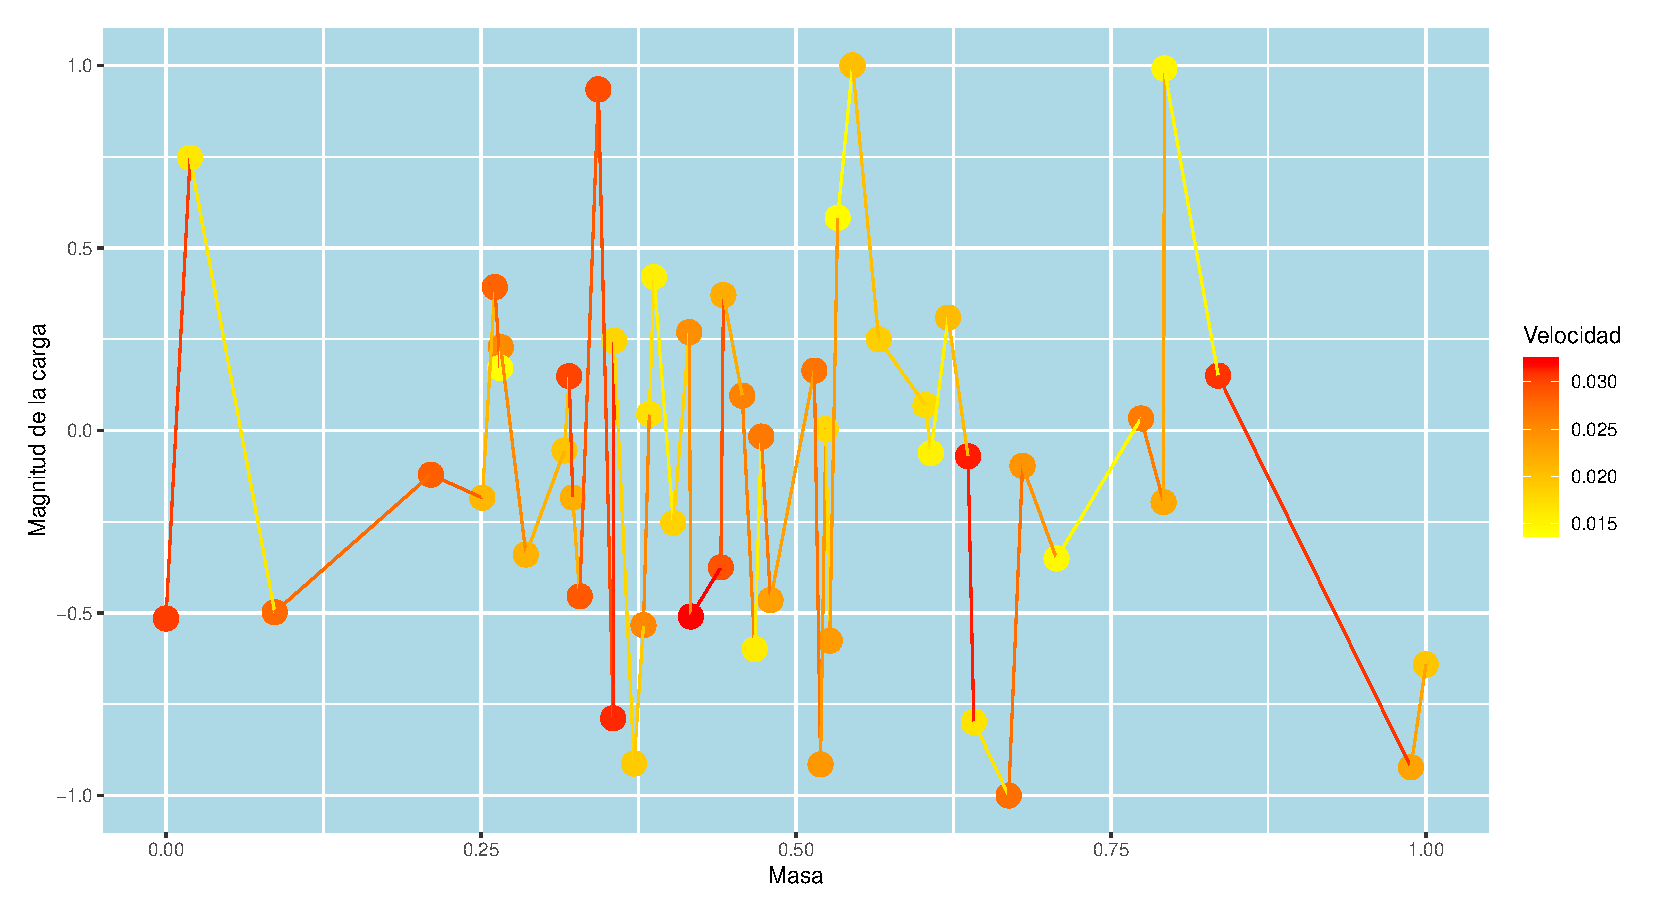
\includegraphics[width=120mm]{resultados.eps}
\caption{Comparaci\'on de las velocidades de las part\'iculas en relaci\'on de su masa y su magnitud de carga}
\label{fig:resultados}
\end{figure}

\bibliographystyle{plainnat}
\bibliography{Bibliografias}
\end{document}